\newpage
\section{Proie}

\begin{figure}[h]
    \centering
    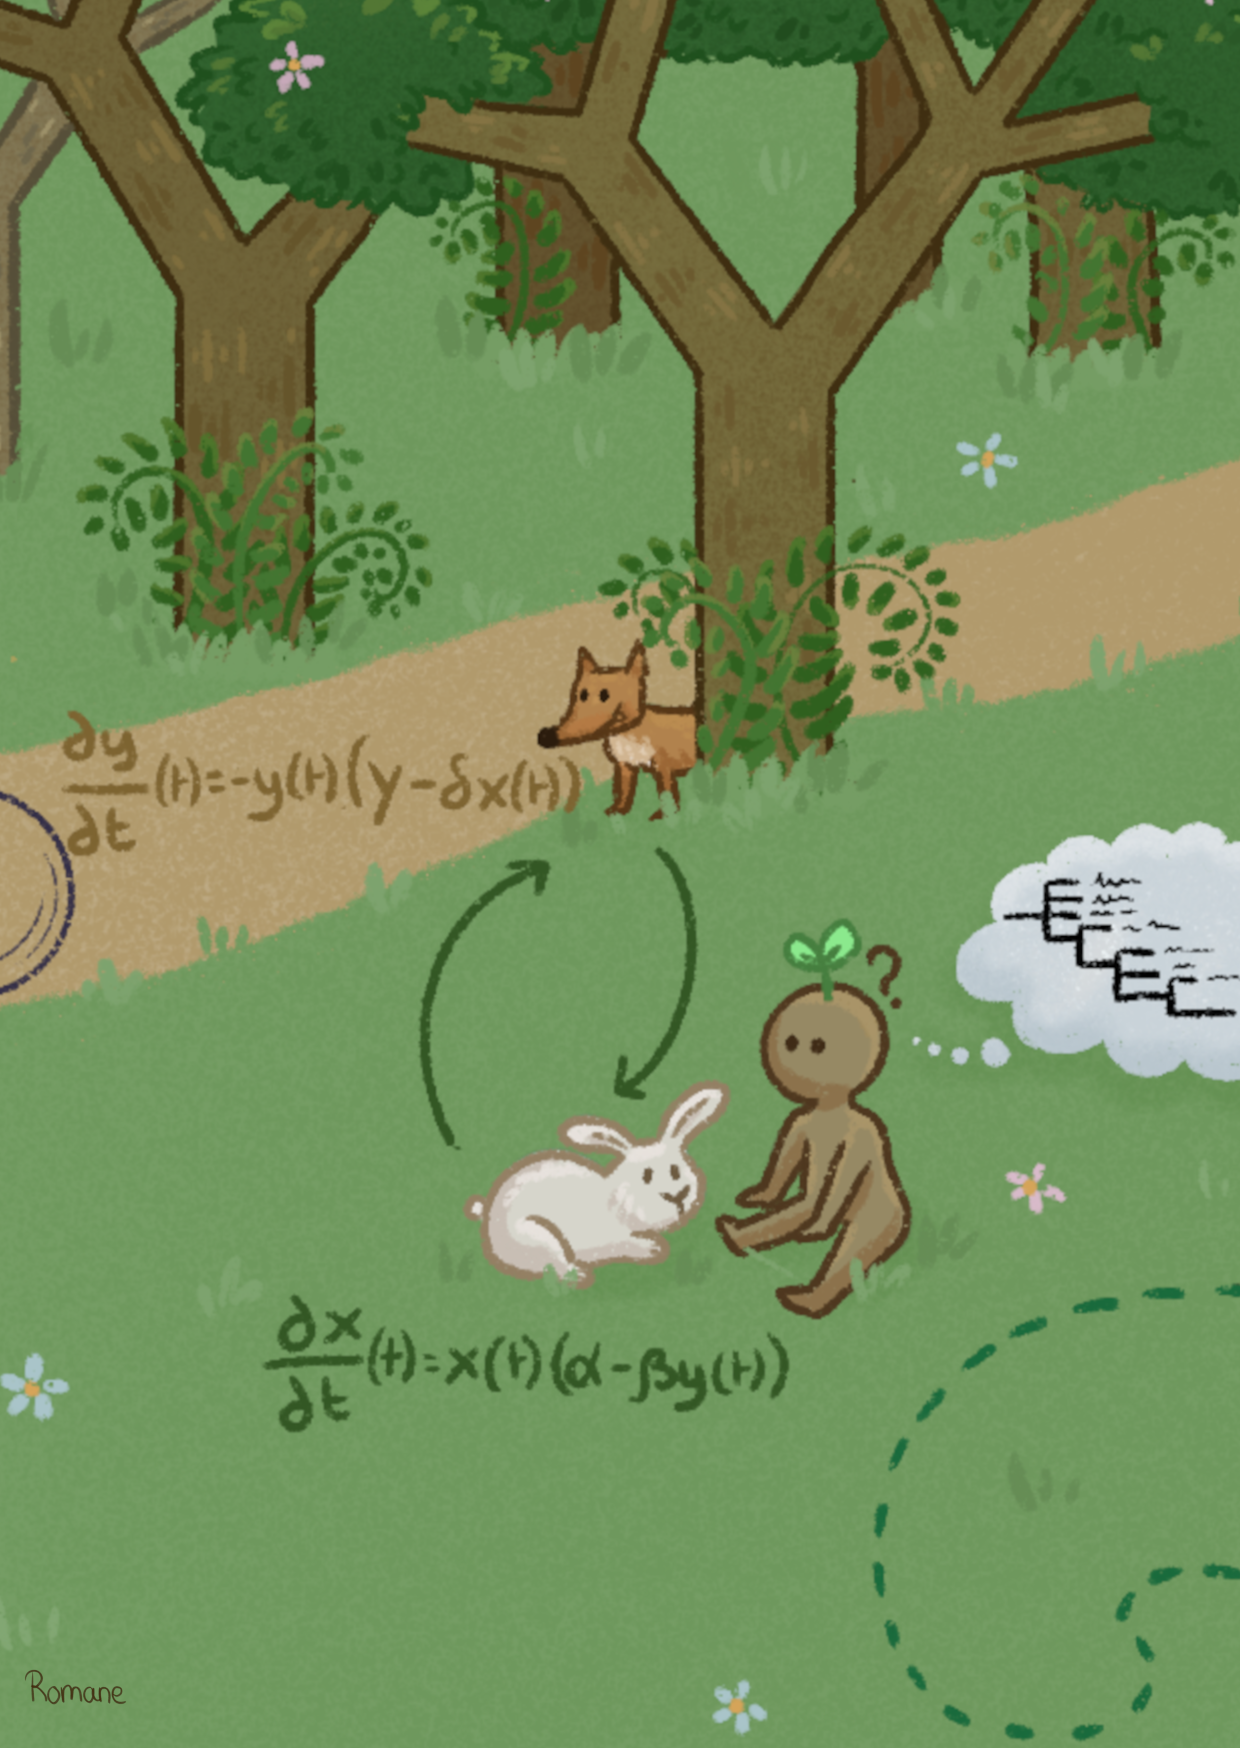
\includegraphics[height=0.5\textheight]{Cartes_postales/carte09-proie.png}\label{fig:c09}
    \caption{Carte postale: Proie}
\end{figure}

Sais-tu qu'on peut modéliser l'évolution des populations de lapins et renards? Lorsqu'il y a beaucoup de lapins, les renards trouvent facilement de la nourriture et leur population augmente. Mais plus il y a de renards, plus les lapins sont mangés et donc le nombre de lapins finit par diminuer. Les renards ont alors plus de difficultés à se nourrir et leur population baisse à son tour. Les lapins, ayant moins de prédateurs, peuvent ensuite se multiplier à nouveau, et le cycle recommence. Les équations ci-dessous permettent de formaliser ce cycle:

\[
\frac{dR(t)}{dt}=-R(t)(a-bL(t))
\]
\newline
\[
\frac{dL(t)}{dt}=L(t)(c-dR(t))
\]

Ce cycle très célèbre est appelé le modèle proie-prédateur et il est très utile pour étudier des populations. Lorsqu'on étudie des populations, on va souvent rencontrer un équilibre stable, le nombre de lapins et renards va se stabiliser autour d'une certaine valeure. Plus l'environnement et les conditions de survie sont stable, plus l'équilibre est durable. Et si les paramètres changent brutalement, comme avec l'arrivée d'une maladie, cet équilibre va se rompre et on va atteindre un nouvel équilibre stable, après une période de grands changements.